\documentclass{standalone}
\usepackage{tikz}
\usetikzlibrary{positioning,shapes,shadows,arrows}

\begin{document}
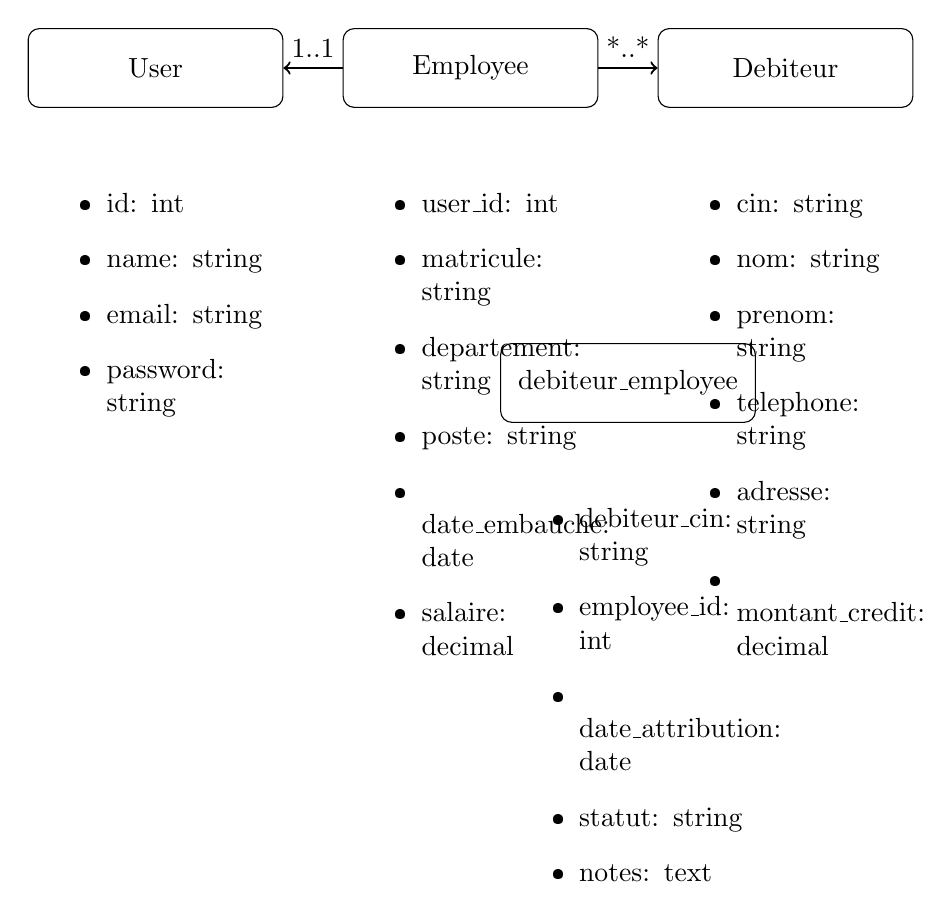
\begin{tikzpicture}[
    class/.style={rectangle, draw, rounded corners, minimum width=3cm, minimum height=1cm, text centered, text width=3cm},
    relation/.style={->, thick},
    attribute/.style={text width=3cm}
]

% Classes
\node[class] (user) at (0,0) {User};
\node[class] (employee) at (4,0) {Employee};
\node[class] (debiteur) at (8,0) {Debiteur};

% Attributes
\node[attribute, below=0.5cm of user] {
    \begin{itemize}
        \item id: int
        \item name: string
        \item email: string
        \item password: string
    \end{itemize}
};

\node[attribute, below=0.5cm of employee] {
    \begin{itemize}
        \item user\_id: int
        \item matricule: string
        \item departement: string
        \item poste: string
        \item date\_embauche: date
        \item salaire: decimal
    \end{itemize}
};

\node[attribute, below=0.5cm of debiteur] {
    \begin{itemize}
        \item cin: string
        \item nom: string
        \item prenom: string
        \item telephone: string
        \item adresse: string
        \item montant\_credit: decimal
    \end{itemize}
};

% Relations
\draw[relation] (employee) -- node[above] {1..1} (user);
\draw[relation] (employee) -- node[above] {*..*} (debiteur);

% Pivot table
\node[class] (pivot) at (6,-4) {debiteur\_employee};
\node[attribute, below=0.5cm of pivot] {
    \begin{itemize}
        \item debiteur\_cin: string
        \item employee\_id: int
        \item date\_attribution: date
        \item statut: string
        \item notes: text
    \end{itemize}
};

\end{tikzpicture}
\end{document} 